\documentclass[a4paper,12pt]{article}


\newcommand{\diepteglb}{../../}

\newcommand{\diepte}{./}

%%%%%%%%%%%%%%%%%%%%%%%%%%%%%%%%%%%%%%%%%%%%%%%%%%%%%%%%%%%%%%%%%%%%%%%%%%%%%%%%%%%%%%%%%%%%%%%%%%%%%%%%%%%%%%%%%%%%%%%%%%%%%%%
%Packages en commands
\input{\diepteglb/includes/packages}
\input{\diepteglb/includes/command}
%%%%%%%%%%%%%%%%%%%%%%%%%%%%%%%%%%%%%%%%%%%%%%%%%%%%%%%%%%%%%%%%%%%%%%%%%%%%%%%%%%%%%%%%%%%%%%%%%%%%%%%%%%%%%%%%%%%%%%%%%%%%%%%
%Paginastijl
%\input{\diepteglb/includes/pagestyleAM}
%%%%%%%%%%%%%%%%%%%%%%%%%%%%%%%%%%%%%%%%%%%%%%%%%%%%%%%%%%%%%%%%%%%%%%%%%%%%%%%%%%%%%%%%%%%%%%%%%%%%%%%%%%%%%%%%%%%%%%%%%%%%%%%
\setlength{\parindent}{0cm}

\begin{document}

\section*{Oefeningen}

\section{Druk uit in radialen:}

\begin{enumerate}
\item $108,17^\circ$ 
\item $12^\circ 40' 33''$ 
\item $190$ gon
\end{enumerate}

Oplossingen: $1,887923$ rad; $0,221235$ rad; $2,984513$ rad (of ook: $\frac{19}{20}\pi$ rad)\\

\section{Reken uit:}

\begin{enumerate}
\item $267,83^\circ - 117,85^\circ$
\item $12^\circ 02' 58'' + 4^\circ 13' 07''$
\item $\frac{5}{3}\pi$ rad - $5^\circ 12' 57''$ (in radialen)
\item $15,15$ gon + $15,15^\circ$ (in decimale graad)
\end{enumerate}

Oplossingen: $149,98^\circ$; $16^\circ 16' 05''$; $5,144954$ rad; $31,9833$ gon

\newpage

\section{Rekenen met driehoeken:}

\begin{enumerate}
\item Om de hoogte van een mast te bepalen plaatst een landmeter een theodoliet in het punt $P$ op een hoogte $h=1,65$ m. Ze meet dan de hoeken $\alpha$ en $\beta$ met de horizontale: $\alpha=78,12^\circ$ en $\beta=4,71^\circ$.\\
    Bereken de hoogte $H$ van de mast.
    
\begin{figure}[h]
\begin{center}
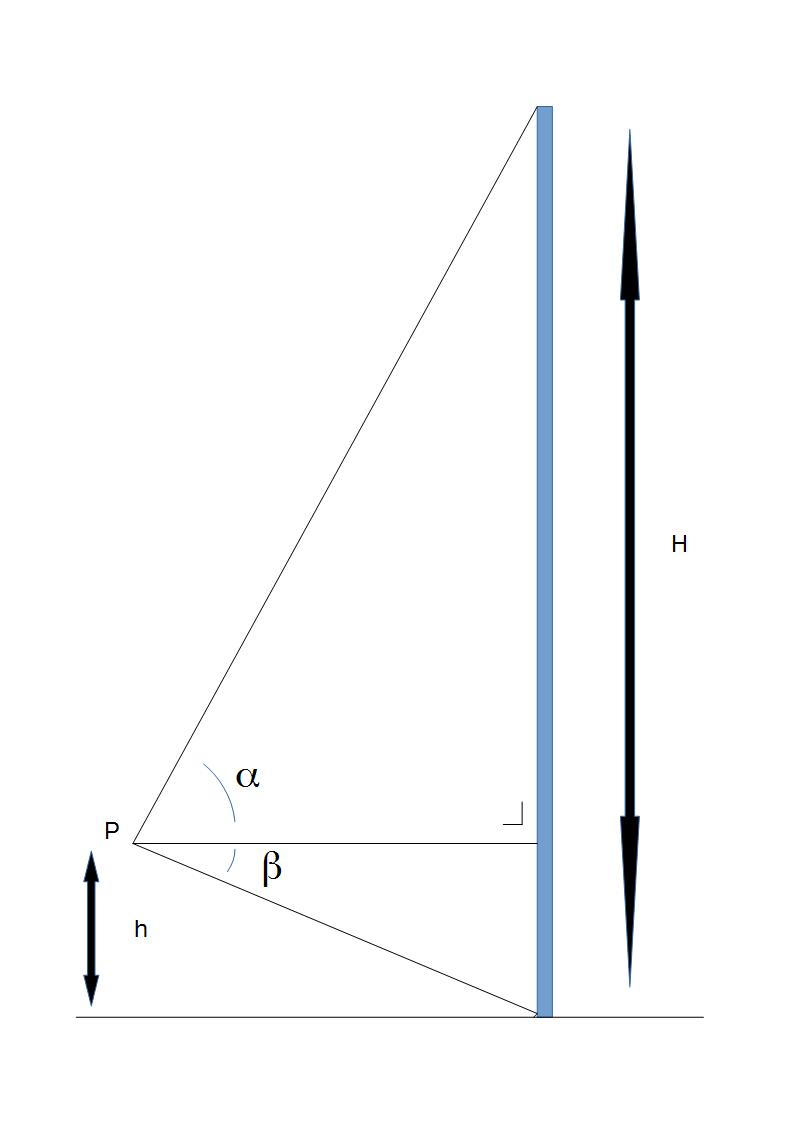
\includegraphics[scale=0.30]{\diepte/figures/oefn-mast.jpg}
\end{center}
\end{figure}

Oplossing: $H=96,85$ m

\item De lengte van elke zijde van de gegeven driehoek zijn gekend: $a=53$ cm, \\ $b=18$ cm en $c=41$ cm.\\
Bereken de hoek $\alpha$.

\begin{figure}[h]
\begin{center}
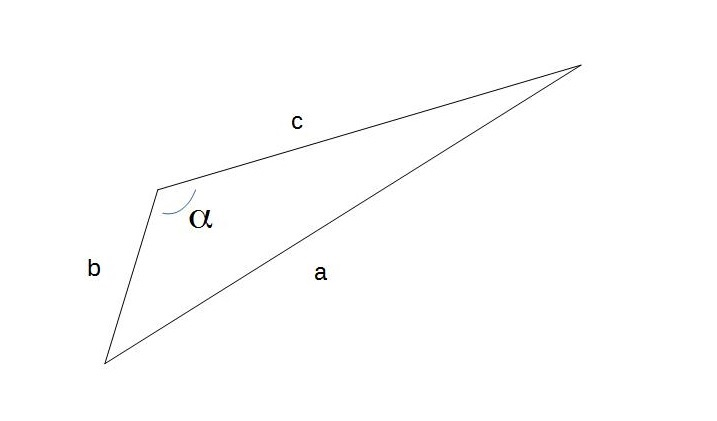
\includegraphics[scale=0.45]{\diepte/figures/oef-driehoek-1.jpg}
\end{center}
\end{figure}

Oplossing: $\alpha=123,01^\circ$ 

\item Bereken de lengte van zijde $c$ van de gegeven driehoek.\\
Gegevens: $a=13$ mm, $b=20$ mm, $\alpha=21^\circ$. 

\begin{figure}[h]
\begin{center}
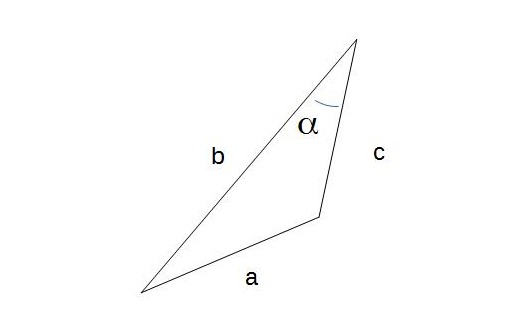
\includegraphics[scale=0.65]{\diepte/figures/oef-driehoek-2.jpg}
\end{center}
\end{figure}

Oplossing: $c=7,83$ mm

\item Op de figuur is een schets van een stuk weiland met de gekende gegevens weergegeven. \\
Bereken de lengte van zijde $d$ en de hoeken $\alpha$ en $\beta$.

\begin{figure}[h]
\begin{center}
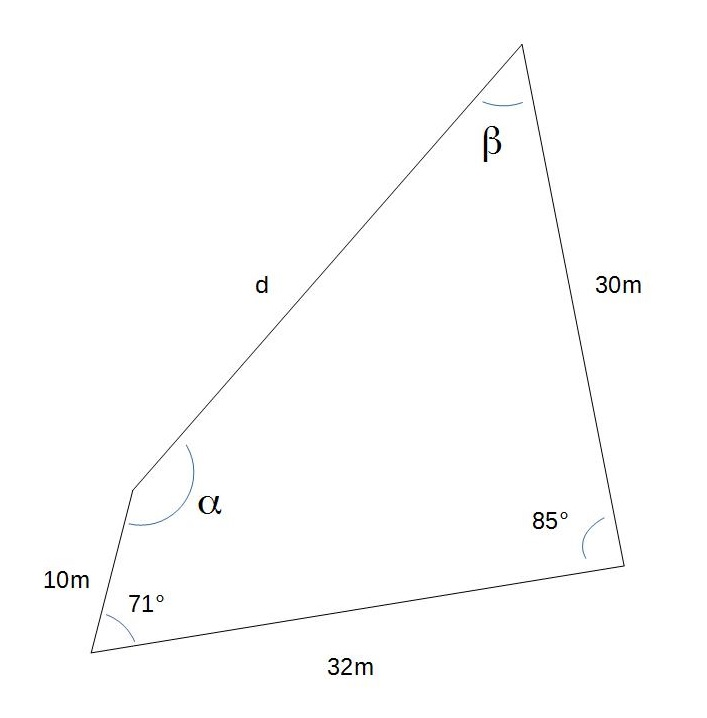
\includegraphics[scale=0.45]{\diepte/figures/oef-driehoek-3.jpg}
\end{center}
\end{figure}

Oplossing: $d=33,17$ m; $\alpha=147,02^\circ$; $\beta=56,98^\circ$

\end{enumerate}

\end{document}
